\chapter{Capitulo 6. Aplicaciones y productos fabricados por medio del proceso}
\label{Punto 6. Aplicaciones}
\section{AFP}
Las capacidades del proceso AFP, así como las ventajas que ofrece, lo hacen un buen candidato para ser utilizado en la fabricación de productos para diversas industrias:
\begin{itemize}
    \item Aeroespacial: el AFP se utiliza ampliamente en la industria aeroespacial para fabricar componentes de aeronaves, como largueros de alas, paneles de fuselaje y mamparos.
    \begin{figure}[H]
        \centering
        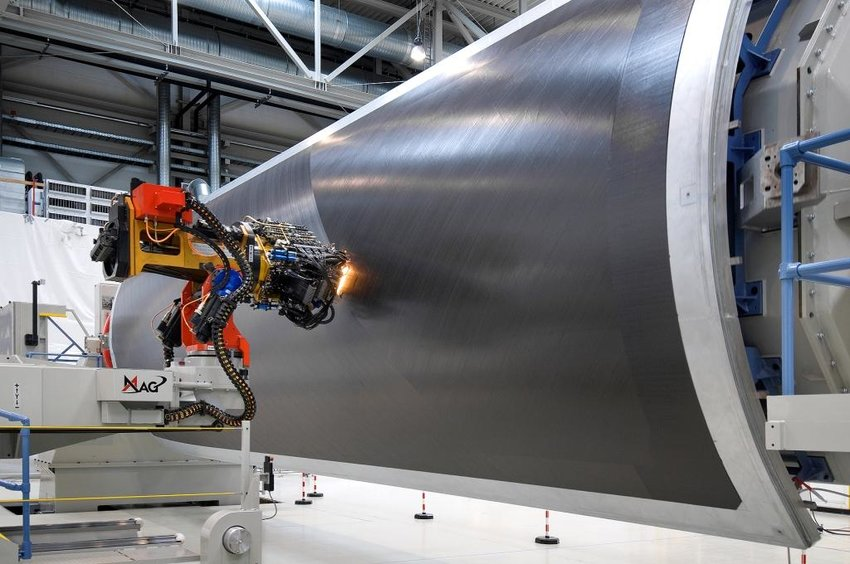
\includegraphics[width=0.75\linewidth]{Fuselaje hecho con AFP.png}
        \caption{Tapa de CFRP (Carbon-fiber-reinforced polymers) para uso aeroespacial}
        \label{fig:enter-label}
    \end{figure}
    \item Automotriz: AFP se puede utilizar para fabricar piezas compuestas para la industria automotriz, como paneles de carrocería, componentes de transmisión y piezas de suspensión.
    \begin{figure}[H]
        \centering
        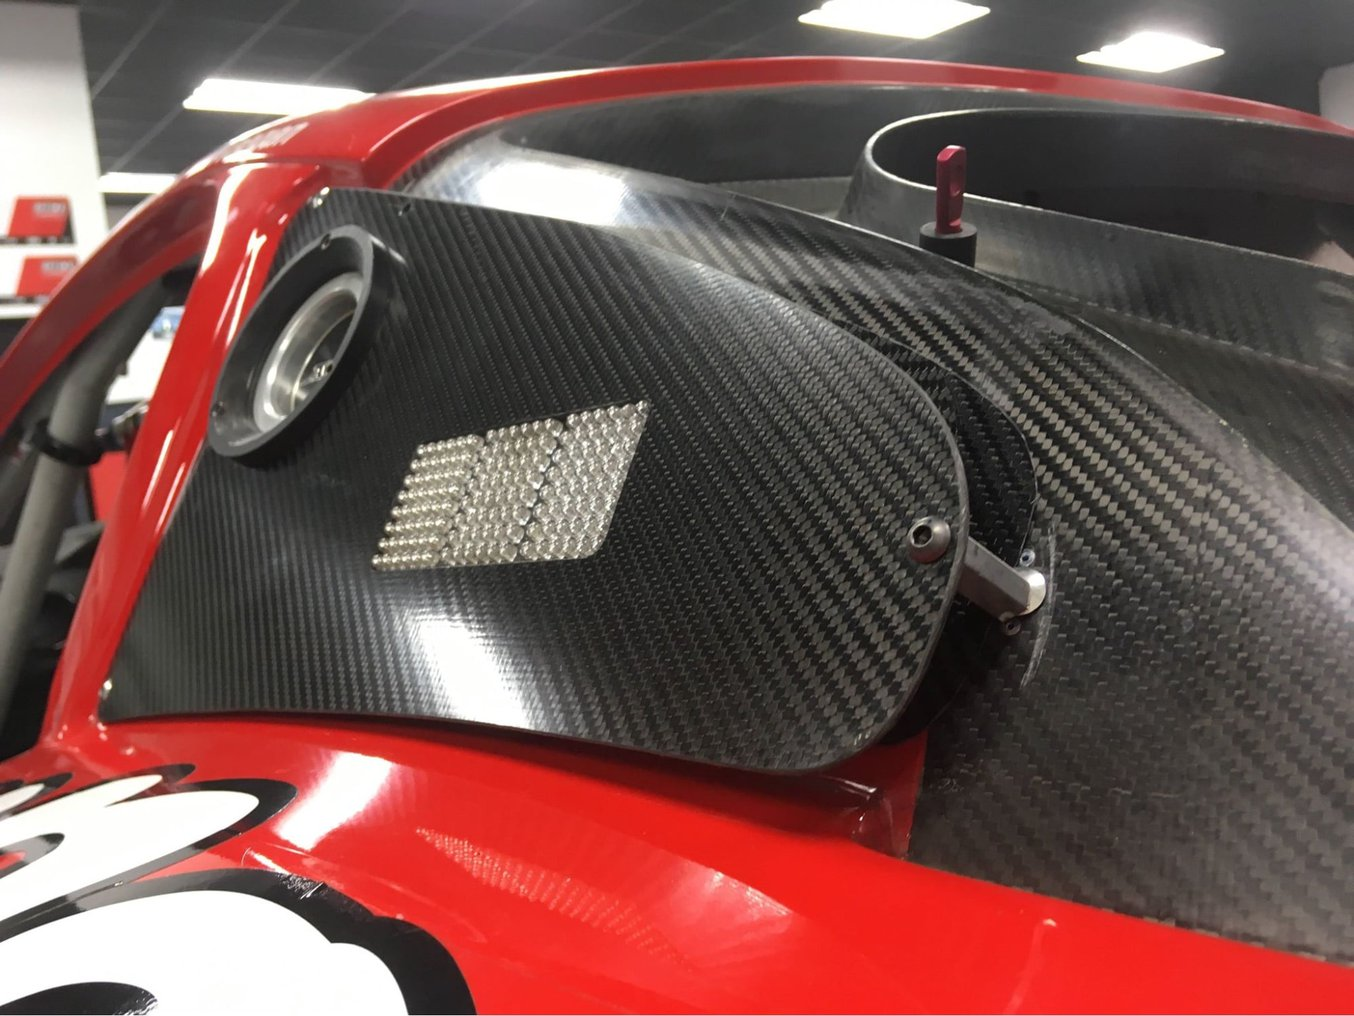
\includegraphics[width=0.5\linewidth]{Pieza de carroceria.png}
        \caption{Pieza de carrocería hecha a base de fibra de carbono}
        \label{fig:enter-label}
    \end{figure}
    \item Construcción: El AFP se puede utilizar para fabricar materiales compuestos para su uso en la construcción, como tableros de puentes, vigas y columnas.
    \item Energía eólica: la AFP se puede utilizar para fabricar palas compuestas de turbinas eólicas, que suelen ser más largas y flexibles que las palas tradicionales.
    \item Artículos deportivos: el AFP se puede utilizar para fabricar materiales compuestos para su uso en artículos deportivos, como palos de golf, raquetas de tenis y esquís.
    \begin{figure}[H]
        \centering
        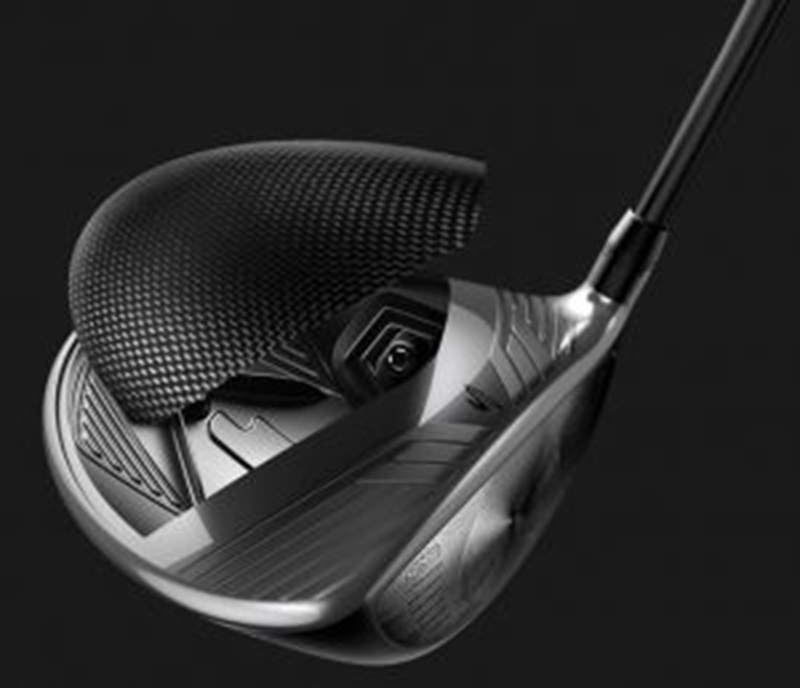
\includegraphics[width=0.5\linewidth]{Articulo deportivo.png}
        \caption{Articulo deportivo fabricado con un material compuesto}
        \label{fig:enter-label}
    \end{figure}
    \item Marina: AFP se puede utilizar para fabricar materiales compuestos para su uso en la industria marina, como cascos de barcos y barcos.
    \item Médico: La AFP se puede utilizar para fabricar materiales compuestos para su uso en dispositivos médicos, como dispositivos implantables y prótesis.
    \item Productos de consumo: la AFP se puede utilizar para fabricar materiales compuestos para su uso en productos de consumo, como productos electrónicos y electrodomésticos.
\end{itemize}
Esta tecnología de laminado es la utilizada para fabricar el cono de cola del avión Airbus A350 XWB.
\begin{figure}[H]
        \centering
        \includegraphics[width=0.70\linewidth]{imagenes/cono de cola A350.png}
        \caption{Fabricación de cono de cola del A350 XWB}
        \label{fig:enter-label}
\end{figure}
    
\section{ATL}

Las aplicaciones típicas en la industria aeroespacial son:
\begin{itemize}
    \item Superficies de control con contornos suaves.
    \begin{figure}[H]
        \centering
        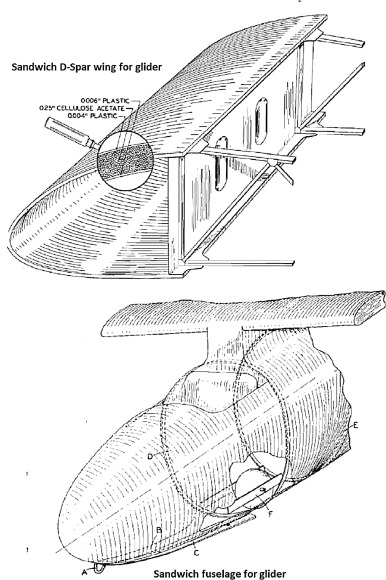
\includegraphics[width=0.35\linewidth]{Superficies de control.png}
        \caption{Componentes estructurales hechos con un material compuesto}
        \label{fig:enter-label}
    \end{figure}
    \item Paneles de fuselaje contorneados.
    \item Secciones de cañón de fuselaje completo.
\begin{figure}[H]
    \centering
    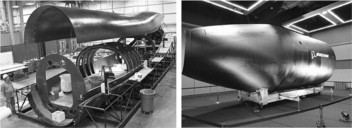
\includegraphics[width=0.8\linewidth]{Secciones de fuselaje.png}
    \caption{Secciones de fuselaje}
    \label{fig:enter-label}
\end{figure}
    \item Carenados contorneados.
    \item Revestimientos de góndola.
    \item Cubiertas/adaptadores de carga útil.
    \item Ejes estructurales (rectos y contorneados).  
    \item Componentes de alas y empenaje.
    \begin{figure}[H]
        \centering
        \includegraphics[width=0.7\linewidth]{imagenes/componente estructural.png}
        \caption{Componente estructural fabricado en ATL}
        \label{fig:enter-label}   
    \end{figure}
\end{itemize}
Si se requiere más contorno, se requeriría una máquina personalizada.

\section{Deposición automática de fibras en la industria aeronáutica}
Debido a las capacidades de este proceso, la industria aeronáutica hace uso de la deposición automática de fibras para la fabricación de múltiples piezas, algunas de las empresas que utilizan este proceso son:
\begin{itemize}
    \item Boeing
    \item Airbus
    \item Spirit Aerosystems
    \item Dassault Aviation
    \item Embraer
    \item GKN Aerospace
\end{itemize}




\textbf{}